\documentclass[11pt]{article}
\usepackage[margin=1in]{geometry}
\usepackage{amsmath,amssymb}
\usepackage{lmodern}
\usepackage[T1]{fontenc}
\usepackage{enumitem}
\usepackage{microtype}
\usepackage{tikz}
\usetikzlibrary{arrows.meta,angles,quotes,calc,decorations.pathreplacing,patterns}

\title{2015 F=ma Exam Review}
\author{Nathan P.}
\date{January 21, 2026}

\begin{document}
\maketitle

\section*{Problem 4}
Writing out the equations shows you the exact slope and $y$-intercept of the $a$ vs.\ $F$ graph when $\mu_k$ is in effect.

\section*{Problem 6}
Collisions don't change the center of mass velocity: $v_{cm}$ is constant regardless of elastic/inelastic collisions.

\section*{Problem 9}
The key idea was using the Pythagorean theorem to relate the perpendicular final momentums with the initial momentum (hypotenuse).

\section*{Problem 10}
Fact: $\Delta K$ cannot be positive in a normal collision (like the last question), so that eliminates several answer options.
Just plug in the numbers and see that it's inelastic.

\section*{Problem 13}
E is the trap: for circular motion (regardless of whether it's uniform or not), the radial component of acceleration always points towards the center, so the acceleration cannot point out of the circle whatsoever.
Thinking in terms of net radial and tangential components might make things easier. Be flexible in changing the way you break components up.

\section*{Problem 17}
F=ma always has a question that seems very hard to solve but it's dimensional analysis.
It's independent of $h/r$ for some reason.

\section*{Problem 18}
Power $\to$ log-log.
Exponential $\to$ log-linear.
Since the log $y$-linear $x$ graph is linear, it must be exponential ($y$-intercept at $\ln a$).

\section*{Problem 19}
Consider a point on the lower side. There is extra pressure from the $2x$ column of water higher on the other side:
\[
F=PA=\rho ghA=\rho g(2x)A=ma=\rho LAa,
\]
so $\rho A$ cancels and $2gx=La$, so
\[
\omega=\sqrt{\frac{2g}{L}}.
\]
The restoring force is due to the weight of the $2x$ of water, and this force accelerates the entire mass of water, so we use $m$ of the whole column.
Guessing is viable for this question because you can eliminate 3 options just with dimensional analysis and guess based on $f$ usually having $1/2\pi$.

\begin{center}
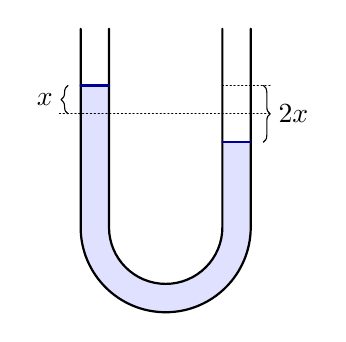
\begin{tikzpicture}[scale=0.9, line cap=round, line join=round, >={Stealth[length=2mm]}]
  % U-tube, left side up by x, right side down by x
  \fill[blue!12] (0,2.6) -- (0,0.6) arc[start angle=180, end angle=360, radius=1.2] -- (2.4,1.8) -- (2.0,1.8) -- (2.0,0.6) arc[start angle=360, end angle=180, radius=0.8] -- (0.4,2.6) -- cycle;
  \draw[thick] (0,3.4) -- (0,0.6) arc[start angle=180, end angle=360, radius=1.2] -- (2.4,3.4);
  \draw[thick] (0.4,3.4) -- (0.4,0.6) arc[start angle=180, end angle=360, radius=0.8] -- (2.0,3.4);
  \draw[thick, blue!60!black] (0,2.6) -- (0.4,2.6);
  \draw[thick, blue!60!black] (2.0,1.8) -- (2.4,1.8);
  \draw[densely dotted] (-0.3,2.2) -- (2.7,2.2);
  \draw[decorate, decoration={brace, raise=2pt}] (-0.1,2.2) -- (-0.1,2.6) node[midway, left=4pt] {$x$};
  \draw[decorate, decoration={brace, mirror, raise=2pt}] (2.5,1.8) -- (2.5,2.6) node[midway, right=4pt] {$2x$};
  \draw[densely dotted] (2.0,2.6) -- (2.7,2.6);
\end{tikzpicture}
\end{center}

\section*{Problem 22}
It'll be no slip when $\theta$ is small, and there's no energy loss at $90^\circ$ because it's in free fall.
An open question: $\mu_k=\mu_s$, so the slipping gradually increases. There should not be a discontinuity in the $E$ vs.\ $\theta$ graph.
Fact: not all of friction does work; $W_f$ is not simply $-fd$.

\section*{Problem 24}
Key idea: $\sigma=F/A$, so $F_{T,\max}=\sigma A$. Plugging that into the equation for the velocity of a transverse wave on a string, we find that
\[
v=\sqrt{\frac{\sigma}{\rho}},
\]
meaning the speed of a wave on the string depends only on properties of the material, not its geometry.

\end{document}
